\documentclass[11pt]{article}
\usepackage{acl2016}
\usepackage{amsmath}
\usepackage{times}
\usepackage{latexsym}
\usepackage{color}
\usepackage{booktabs}
\usepackage{subfig}
\usepackage{tikz}
\usetikzlibrary{bayesnet}

\newcommand{\secref}[1]{Section~\ref{sec:#1}}
\newcommand{\figref}[1]{Figure~\ref{fig:#1}}
\newcommand{\algref}[1]{Algorithm~\ref{alg:#1}}
\newcommand{\tabref}[1]{Table~\ref{tab:#1}}
\newcommand{\mattnote}[1]{\textcolor{red}{NOTE: #1}}
\newcommand{\blank}{\underline{\hspace{.5cm}}}
\newcommand{\predicate}[1]{\ensuremath{\textsc{#1}}}
\newcommand{\entity}[1]{\ensuremath{\textsc{#1}}}

\newcommand{\true}[0]{\predicate{true}}
\newcommand{\false}[0]{\predicate{false}}

%\aclfinalcopy % Uncomment this line for the final submission
%\def\aclpaperid{***} %  Enter the acl Paper ID here

\title{Combining formal and distributional models of predicate semantics}

\author{}%Matt Gardner and Jayant Krishnamurthy\\
%Allen Institute for Artificial Intelligence\\
%Seattle, Washington, USA\\
%{\tt \{mattg,jayantk\}@allenai.org}}

\date{}

\begin{document}

\maketitle

\begin{abstract}

  We consider the problem of learning models of predicate (category and
  relation) semantics using both distributional information and structured
  information contained in a formal knowledge base.  Most previous approaches
  to modeling predicate semantics have either been purely distributional (such
  as word2vec and knowledge base embedding methods) or purely formal (such as
  most semantic parsers).  Distributional approaches have very broad coverage,
  but lack the compositional, logical semantics used by semantic parsers, and
  it has so far been difficult to combine the benefits of both of these
  techniques.

  In this paper, we present a method that incorporates logical statements
  derived from a knowledge base into distributional models of categories and
  relations.  Instead of mapping a phrase to a single logical statement, as
  done by semantic parsers, our method uses logical statements as features
  added to distributional models of words, allowing the model to learn that
  Freebase entities that are "honchos" are people, not buildings, and that they
  are frequently CEOs or film producers.  We use these models in an
  open-vocabulary semantic parsing task, showing a 62\% relative improvement in
  mean average precision over a distributional-only model.

\end{abstract}

\section{Introduction}

How should a computer program represent the meaning of a word or a phrase?  The
answer to this question has a long and rich history.  Motivated by Harris's
distributional hypothesis~\cite{harris-1954-distributional-hypothesis}, much
work has been put into representing words as collections of the contexts in
which they appear.  Recent work with neural networks and word embeddings have
shown that these representations can be very useful for a number of natural
language processing tasks (see, e.g., the work Mikolov et
al.~\shortcite{mikolov-2013-word2vec} and papers that cite them).  This
approach to modeling semantics is appealing because word embeddings can be
trained on unlabeled text, allowing for very broad coverage, although shallow,
semantics.

\begin{figure*}[ht]
  \small
  \begin{minipage}{0.28\linewidth}
    \textbf{Input Text}\\Italian architect Andrea Palladio
  \end{minipage}
%
  ~~ $\rightarrow$ ~~~~~~
%
  \begin{minipage}{0.7\linewidth}
    \textbf{Logical Form}\\
    $\predicate{architect}(\entity{Palladio})~\land~\predicate{architect\_N/N}(\entity{Italy}, \entity{Palladio})$
  \end{minipage}

  \vspace{.2in}
  \begin{minipage}{0.5\linewidth}
    \textbf{Category models}\\
    \begin{tabular}{@{}lll}
      \predicate{architect}: & $\theta$: &[.2, -.6, \ldots] \\
      & $\omega$: & \textsc{type:architect} $\rightarrow$ .52 \\
      &           & \textsc{type:designer} $\rightarrow$ .32 \\
      &           & \textsc{nationality:Italy} $\rightarrow$ .20 \\
      &           & $\cdots$
    \end{tabular}
  \end{minipage}
  \begin{minipage}{0.5\linewidth}
    \textbf{Relation models}\\
    \begin{tabular}{@{}lll}
      \predicate{architect\_N/N}: & $\theta$: &[-.9, .1, \ldots] \\
      & $\omega$: & \textsc{/person/nationality\textsuperscript{-1}} $\rightarrow$ .29 \\
      &           & \textsc{/structure/architect} $\rightarrow$ .11 \\
      &           & \textsc{/person/ethnicity\textsuperscript{-1}} $\rightarrow$ .05 \\
      &           & $\cdots$
    \end{tabular}
  \end{minipage}

  \vspace{.1in}
  \begin{minipage}{0.5\linewidth}
    \textbf{Entity models}\\
    \begin{tabular}{@{}lll}
      \predicate{Palladio}: & $\phi$: &[.15, -.8, \ldots] \\
      & $\psi$: & \textsc{type:architect} $\rightarrow$ 1 \\
      &           & \textsc{type:designer} $\rightarrow$ 0 \\
      &           & \textsc{nationality:Italy} $\rightarrow$ 1 \\
      &           & $\cdots$
    \end{tabular}
  \end{minipage}
  \begin{minipage}{0.5\linewidth}
    \textbf{Entity pair models}\\
    \begin{tabular}{@{}lll}
      \predicate{(Italy, Palladio)}: & $\phi$: &[-.8, .2, \ldots] \\
      & $\omega$: & \textsc{/person/nationality\textsuperscript{-1}} $\rightarrow$ 1 \\
      &           & \textsc{/structure/architect} $\rightarrow$ 0 \\
      &           & \textsc{/person/ethnicity\textsuperscript{-1}} $\rightarrow$ 0 \\
      &           & $\cdots$
    \end{tabular}
  \end{minipage}

  \vspace{-.1in}
  \caption{Overview of the components of our model.  Given an input text, we
  use a CCG parser and an entity linker to produce a logical form that is a
  conjunction of predicates involving the entities in the text.  For each
  predicate (both categories and relations), we learn a distributional vector
  $\theta$, as well as weights $\omega$ associated with formal features from
  Freebase (which are shortened to fit in the figure).  For each entity and
  entity pair, we also learn a distributional vector $\phi$, and we extract a
  feature vector $\psi$ from Freebase.  These models are combined to assign a
  probability to the input text, assigning a high probability to the above
  text, and a low probability to ``Italian architect Barack Obama''.}
  \label{fig:overview}
  \vspace{-.1in}
\end{figure*}

At the same time, other researchers have found Montague's ideas about English
as a formal language to be useful~\cite{montague-1974-english-formal-language}.
Modern semantic parsers make use of a model-theoretic semantics that represents
words and phrases as formal predicates.  These predicates are then typically
mapped onto a query over a structured knowledge base, such as
Freebase~\cite{freebase-2008-bollacker}.  This kind of modeling allows semantic
parsers to handle the compositional structure of natural language and to
leverage large, curated knowledge sources to perform various natural language
processing
tasks~\cite{zettlemoyer-2005-ccg,kwiatkowski-2013-ontology-matching,berant-2013-semantic-parsing-qa}.
However, semantic parsers are fundamentally limited by the schema of the
ontology they are trained on---a semantic parser trained with Freebase cannot
even represent words whose meaning has no correlate in the Freebase ontology,
such as ``front-runner'' and ``honcho''.

In this work we introduce models of predicate semantics that combine the
benefits of both distributional and formal approaches.  While there is no
Freebase predicate that corresponds exactly to the meaning of ``honcho'',
Freebase \emph{does} contain many predicates that can \emph{partially}
represent the word.  Our models extract features from Freebase that are
correlated with words and phrases seen in natural language text, and learns
weights for those features as additional components of a distributional model
of the word's meaning.

To demonstrate these models, we focus on the task of fill-in-the-blank natural
language queries, such as ``Italian architect \blank{}''.  Similar to many
current semantic parsers, we first convert this natural language query into a
logical form: $\lambda x. \predicate{architect}(x) \land
\predicate{architect\_N/N}(\entity{Italy},
x)$.\footnote{\predicate{architect\_N/N} represents a noun-compound
relationship between two entities mediated by the word ``architect'', as in
``Italian architect Andrea Palladio''.  This is in contrast to, e.g.,
\predicate{'s\_architect} or \predicate{architect\_of}, both of which also are
mediated by ``architect'', but through different syntax.  N/N is how
CCG~\cite{steedman-2006-ccg} represents a noun compound.} A typical semantic
parser (e.g., that of Kwiatkowski et
al.~\shortcite{kwiatkowski-2013-ontology-matching}) would then try to map this
logical form to a single Freebase query, likely involving
(\predicate{/people/person/nationality}: \entity{Italy}) and
(\predicate{/type/object/type}: \entity{/architecture/architect}).  Instead of
restricting ourselves to modeling only what can be represented as a Freebase
query, we follow Krishnamurthy and
Mitchell~\shortcite{krishnamurthy-2015-semparse-open-vocabulary} in learning a
model for each predicate that can give a \emph{score} to potential arguments.
The model for \predicate{architect}, e.g., should give high scores to
\entity{Andrea Palladio} and \entity{Frank Lloyd Wright}, and low scores to
\entity{Italy}, \entity{BarackObama}, etc.  However, while the models of
Krishnamurthy and Mitchell are purely distributional, using Freebase only as a
means of finding entities in text, we inject additional information from
Freebase into the models for each predicate.  The model we learn for
\predicate{architect} has a \emph{feature} capturing the fact that an entity
has the type \entity{/architecture/architect} in Freebase, and the model for
\predicate{architect\_N/N} has a \emph{feature} capturing whether the first
argument is the country of nationality of the second argument.  An overview of
the components of our model is given in \figref{overview}.

This is a new kind of predicate semantics.  It is distributional---part of the
model is still trained in a manner very similar to word2vec---yet it is also
formal.  However, instead of committing to a single Freebase query to represent
a phrase, as traditional formal approaches do, our models are flexible,
encoding many possible Freebase queries as features that can give hints to the
model.  Thus words that would be impossible to represent as a single Freebase
query can still benefit from the information contained in Freebase---our model
for ``front-runner'' learns that acceptable entities are politicians, even
though there is no exact encoding of ``front-runner'' in Freebase.

The rest of this paper is organized as follows.  In \secref{background}, we
describe the relevant background necessary to understand the models we propose,
and we situate our model in the context of related work.  In \secref{method},
we give a formal description of our models of predicate semantics.  In
\secref{evaluation}, we present experimental results on fill-in-the-blank
natural language query task.  Using web text linked to Freebase as our training
and test data, we show a 62\% relative improvement over prior work, giving a
new state-of-the-art result on this dataset.  In \secref{discussion}, we give a
detailed discussion of the benefits and drawbacks of the models we have
proposed.  We then conclude in \secref{conclusion}.

\section{Background}
\label{sec:background}

Our proposed method is best viewed as the addition of SFE
features~\cite{gardner-2015-sfe} to Krishnamurthy and
Mitchell's~\shortcite{krishnamurthy-2015-semparse-open-vocabulary}
open-vocabulary semantic parser.  Accordingly, in this section we briefly
describe both of these techniques, as well as give a short overview of other
closely related work.

\subsection{Open-vocabulary semantic parsing}
\label{sec:jayant-semparse}

Krishnamurthy and
Mitchell~\shortcite{krishnamurthy-2015-semparse-open-vocabulary} introduced a
technique for learning semantic parsers with open predicate vocabularies
(hereafter referred to as K\&M).  Instead of mapping text to Freebase queries,
they applied the matrix factorization semantics used by Riedel et
al.~\shortcite{riedel-2013-mf-universal-schema} in knowledge base completion to
the task of learning predicate semantics in a semantic parser.  This method
assigns truth values to instantiated predicates like
\predicate{architect}(\entity{AndreaPalladio}) in a probabilistic database.
The models K\&M use for the predicates and entities are essentially equivalent
to modern techniques for constructing word embeddings, implicitly factorizing a
cooccurrence matrix between categories and entities, and relations and entity
pairs~\cite{levy-2014-w2v-as-mf}.  This implicit factorization has two sets of
parameters: each predicate (category or relation) has a learned $k$-dimensional
embedding $\theta$, and each entity and entity pair has a learned embedding
$\phi$.  The probability assigned to a category instance $c(e)$ and relation
instance $r(e_1, e_2)$ in the probabilistic database is given by:

\begin{align*}
  P(c(e)) &= \sigma ( \theta_c^T \phi_e ) \\
  P(r(e_1, e_2)) &= \sigma ( \theta_r^T \phi_{(e_1, e_2)} )
\end{align*}

The probability of a predicate instance is the (sigmoided) inner product of the
corresponding predicate and entity embeddings. Thus, predicates with nearby
embeddings will have similar distributions over the entities in their
denotation.  The model is trained using a ranking objective that learns to rank
the observed entities for each query above unobserved entities.  The
probabilistic database produced by these predicate models is then input to a
reasoning system that can handle a subset of first-order logic.

In this paper, we use the system produced by K\&M, changing only the models of
predicate semantics, as described in \secref{method}.  K\&M introduced several
variations of their parser; in this work, we use their query ranking objective,
as it had the best performance, and we evaluate the model they called
``Factorization'', without ensembling it with a clustering baseline.

\subsection{Subgraph feature extraction}

\begin{figure}
  {\center
  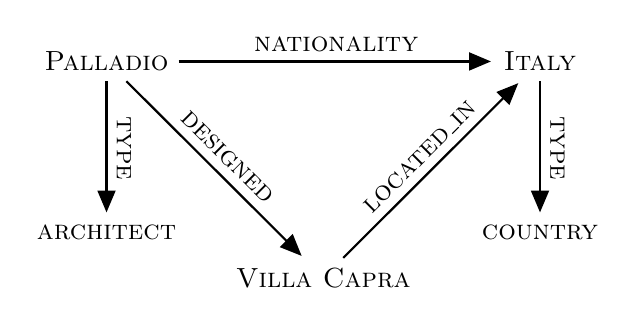
\begin{tikzpicture}[
    ->,
    shorten >=1pt,
    auto,
    node distance=3cm,
    thick,
    main node/.style={draw=none,fill=none}
    ]

    \node[main node] (1) {\entity{Palladio}};
    \node[main node] (2) [right=4cm of 1] {\entity{Italy}};
    \node[main node] (3) [below=1.7cm of 1] {\entity{architect}};
    \node[main node] (4) [below=1.7cm of 2] {\entity{country}};
    \node[main node] (5) [below right=.1cm and .5cm of 3] {\entity{Villa Capra}};

    \path[]
      (1) edge node [sloped, anchor=center, above] {\predicate{nationality}} (2)
      (1) edge node [sloped, anchor=center, above] {\predicate{type}} (3)
      (1) edge node [sloped, anchor=center, above] {\predicate{designed}} (5)
      (2) edge node [sloped, anchor=center, above] {\predicate{type}} (4)
      (5) edge node [sloped, anchor=center, above] {\predicate{located\_in}} (2);
  \end{tikzpicture}
  }
  \textbf{Features between \entity{Palladio} and \entity{Italy}}:\\
  \textless\predicate{nationality}\textgreater\\
  \textless\predicate{designed}, \predicate{located\_in}\textgreater
  \caption{A subset of the Freebase graph, and some example extracted features
  between \entity{Palladio} and \entity{Italy}.  The actual Freebase relations
  and entity identifiers used are modified here to aid readability.}
  \label{fig:sfe}
\end{figure}

Subgraph feature extraction (SFE) is a technique introduced by Gardner and
Mitchell~\shortcite{gardner-2015-sfe} for generating feature matrices over node
pairs in a graph with labeled edges.  Given a pair of nodes in a graph, SFE
performs a search to characterize a subgraph around those two nodes, then
extracts various kinds of features from that subgraph, such as the set of edge
sequences that connect the two nodes.  \figref{sfe} shows an example subgraph,
centered around \entity{Andrea Pallado} and \entity{Italy}, and features that
would be extracted for that entity pair.  Gardner and Mitchell used these
features to perform link prediction in the graph, using characteristics of the
subgraph around two nodes to determine if an edge of a particular type should
exist between those nodes.\footnote{When the graph corresponds to a knowledge
base like Freebase, this task is also known as knowledge base completion.}
Gardner and Mitchell only used these features to model formal KB relations,
however.

We differ from the work done by Gardner and Mitchell in two ways.  First, we
apply these features to models of natural language, instead of formal KB
relations.  There are some non-trivial problems that need to be solved in order
to make this work, which will be discussed in \secref{method}.  Second, Gardner
and Mitchell only considered generating feature matrices over node \emph{pairs}
in a graph, with which one can model binary relations.  The natural language
queries we wish to answer also involve unary predicates, or categories.  We
thus extend SFE to also generate feature matrices over \emph{nodes} in a graph,
an extension that is straightforward and is also discussed in more detail in
\secref{method}.

\subsection{Other related work}

There is a large body of other work that is closely related to what is
presented in this paper.  Two recent papers that also attempt to include some
form of structured knowledge into distributional representations are those by
Faruqui et al.~\shortcite{faruqui-2015-retrofitting-word-vectors}, and by
Rockt\"{a}schel et al.~\shortcite{rocktaschel-2015-logical-embeddings}.  A key
difference between their approaches and ours is that they use the structured
information only to modify distributional representations, while we include the
structured information directly in our models, training weights for structured
information jointly with distributional representations.  Also conceptually
similar is the Additive Relational Effects model for knowledge base completion
by Nickel et al.~\shortcite{nickel-2014-are}, which tries to factorize the
residual of a KB tensor that cannot be explained by observable features that
are somewhat similar to the formal features we use in this model.  But while
this model is conceptually similar, it is computationally quite different, and
would be rather difficult to use in the setting we explore in this work.

Our work draws a lot of inspiration from recent work on knowledge base
completion.  We are building on top of work in embedding the entities and
relations in a knowledge
base~\cite{riedel-2013-mf-universal-schema,nickel-2011-rescal,bordes-2013-transe},
as well as work on graph-based methods for reasoning with knowledge
bases~\cite{lao-2010-original-pra,gardner-2014-vector-space-pra,neelakantan-2015-rnn-kbc}.

Lastly, there is an extensive literature on building semantic parsers to answer
questions against a structured knowledge
base~\cite{zettlemoyer-2005-ccg,berant-2013-semantic-parsing-qa,%
kwiatkowski-2013-ontology-matching,krishnamurthy-2012-semantic-parsing}.  The
vast majority of this work is focused on matching natural language text to
statements in a specific ontology, with no hope of assigning meaning to
language that falls outside of that ontology.  Only very recently has there
been work attempting to learn broad coverage meaning representations in
semantic parsers.  In addition to the work by Krishnamurthy and Mitchell which
we extend in this paper, there was recently a nice piece of work by Choi et
al.~\shortcite{choi-2015-semantic-parsing-partial-ontologies}.  The aim of
their work is, like typical semantic parsers, to map text onto a single formal
statement, but they allow some of the predicates to be ``open'' predicates not
contained in the Freebase ontology.  A key difference between their work and
ours is that we score surface logical forms directly, using a weighted
combination of many Freebase queries, instead of trying to map them to a single
Freebase logical form.  Additionally, while their system might learn that
``front-runner'' should be modeled as an open predicate that has no
representation in Freebase, they have no method to assign any further meaning
to that predicate, while our models learn both distributional and formal
information about the meaning of ``front-runner''.

\section{Method}
\label{sec:method}

In this section we present our models of predicate semantics.  In
\secref{formal-and-distributional} we describe how we modify Krishnamurthy and
Mitchell's (K\&M's) semantic parser to include features from a formal knowledge
base.  In \secref{computing-pmi} we describe how we select those features for
each predicate.  The remaining two sections then describe other improvements we
made to K\&M's semantic parsing model: lexicalizing preposition and
noun-compound predicates, and using the Freebase graph to select candidate
entities.

\subsection{Formal features for predicate semantics}
\label{sec:formal-and-distributional}

We inject information from a formal knowledge base into our models of predicate
semantics simply by augmenting the learned distributional feature vectors with
formal features.

For each entity and entity pair in the data we compute an SFE feature vector
$\psi(e)$ and $\psi(e_1, e_2)$.  For entity pairs, the vector $\psi(e_1, e_2)$
is a sparse binary vector containing indicator features for all edge sequences
that connect nodes $e_1$ and $e_2$ in the Freebase graph, up to length 4.
These features are shown for the entity pair (\entity{Palladio},
\entity{Italy}) in the example graph in \figref{sfe}.  For entities, we extract
similar features to form the sparse binary vector $\psi(e)$.  These features
are of two types: (1) edge sequences that begin at node $e$ (up to length two),
and (2) edge sequences that begin at node $e$ along with the node at the end of
the sequence.  For example, all of the features listed in \figref{sfe} for the
entity pair (\entity{Palladio}, \entity{Italy}) are also valid features of type
(1) for the entity \entity{Palladio}, as well as the features
\textless\predicate{type}\textgreater and
\textless\predicate{designed}\textgreater.  Examples of of type (2) features
are \textless\predicate{type}\textgreater:\entity{architect}, and
\textless\predicate{nationality}\textgreater:\entity{Italy}.  Intuitively,
features of type (1) capture the fact that an entity participates in particular
kinds of relations, such as designing architectural structures, while features
of type (2) capture the way an entity is related to particular other entities.
Features of type (2) are very specific, and are most useful in practice when
the entity in the feature is a type node, such as with
\textless\predicate{type}\textgreater:\entity{architect}, though occasionally
features of this type involving other entities are also selected in our feature
selection process.

For each category and relation, we select a subset of the SFE features in the
vectors $\psi$ to have associated weights $\omega_c$ and $\omega_r$.  We then
add the weights $\omega_c$ and $\omega_r$ as parameters to be learned for each
predicate, and we add the feature vectors $\psi(e)$ and $\psi(e_1, e_2)$ as
observed features for each entity and entity pair.  The augmented category and
relation probabilities are as follows:

\begin{align*}
  P(c(e)) &= \sigma ( \theta_c^T \phi_e + \omega_c^T \psi_c(e)) \\
  P(r(e_1, e_2)) &= \sigma ( \theta_r^T \phi_{(e_1, e_2)} + \omega_r^T \psi_r(e_1, e_2) )
\end{align*}
where we have added subscripts on the $\psi$ functions to indicate that each
predicate selects its own set of features from the SFE feature vector $\psi$.

We pause here to note that these features obtained from SFE correspond exactly
to a limited set of horn clauses using the Freebase vocabulary, which in turn
can be seen as Freebase queries that define sets of entities or entity pairs.
By associating a number of these features with each predicate and assigning
them weights, what we are effectively doing is mapping language onto a weighted
combination of possible Freebase statements, instead of onto a single Freebase
query, as is typically done in the semantic parsing literature.  This is a
fundamentally new kind of predicate semantics that has not been used previously
in semantic parsers.

Note also that in our combined model there are now three sets of parameters to
be learned by the semantic parser: (1) $\theta$, low-dimensional distributional
vectors trained for each predicate; (2) $\phi$, low-dimensional distributional
vectors trained for each entity and entity pair; and (3) $\omega$, weights
associated with the selected formal SFE features for each predicate.  All of
these parameters are optimized jointly, using the same ranking objective used
by K\&M.

\subsection{Finding relevant features for each predicate}
\label{sec:computing-pmi}

The feature vectors returned by SFE have dimensionality in the tens of
millions.  We do not have near enough data to train that many parameters for
each of our tens of thousands of predicates, nor do we have enough RAM in our
machines to keep that many parameters in memory.  It is thus necessary to
select some small number of informative features for each predicate.  We do
this using pointwise mutual information (PMI).

PMI measures the strength of association between two variables $x$ and $y$; it
is computed as $\log\frac{p(x,y)}{p(x)p(y)}$.  In our case, we want to
associate predicates with SFE features.  However, our SFE features are for each
\emph{entity} and \emph{entity pair}, not each \emph{predicate}.  To associate
SFE features with predicates, we use the training data to find a mapping from
entities and entity pairs to predicates that they have been seen with in the
data.  For example, the phrase ``Italian architect Andrea Palladio'' is
considered a positive training example for the instantiated predicates
$\predicate{architect}(\entity{Andrea Palladio})$ and
$\predicate{architect\_N/N}(\entity{Italy}, \entity{Andrea Palladio})$.  We
then associate the feature vectors for \entity{Andrea Palladio} and
(\entity{Italy}, \entity{Andrea Palladio}) with the predicates
\predicate{architect} and \predicate{architect\_N/N}, respectively.  For each
predicate $\pi$ and feature $f$, we use these counts to calculate the
probabilities $p(\pi, f)$, $p(\pi)$ and $p(f)$.  After removing features with
counts below some threshold, we pick the $k$ features with the highest PMI
values for each predicate to use in our model.\footnote{We used $k=100$ in this
paper.}

\subsection{Improved logical forms}
\label{sec:better-lfs}

While we largely follow the semantic parsing framework introduced by K\&M, we
made one important change in how logical forms are generated.  For the running
example we have been using this paper, ``Italian architect Andrea Palladio'',
the relation predicate produced by K\&M's system is
$\predicate{N/N}(\entity{Italy}, \entity{Andrea Palladio})$.  \predicate{N/N}
does correctly capture the fact that \entity{Italy} is used syntactically as a
noun modifier of \entity{Andrea Palladio}, but it leaves out the additional
information contained in the syntax that ``architect'' was mediating that
noun-noun dependency.  This means that ``U.S. president Barack Obama'' and
``Italian architect Andrea Palladio'' are both modeled using the same relation
predicate, which leads to a very generic and largely useless model for the
predicate \predicate{N/N}.  By splitting \predicate{N/N} into separate
predicates (\predicate{architect\_N/N} and \predicate{president\_N/N}), we give
the model the opportunity to learn more fine-grained relation semantics, and we
allow our feature selection pipeline to find much more useful features for
relation predicates.  While it would be ideal to use actual dependency
relations to determine which words to add to the predicate in complex noun
phrases, most current parsers treat these kinds of noun phrases as flat, with
all noun modifiers depending directly on the head of the noun phrase.  We
approximate this ideal by simply taking all words in between the two entities
in a noun phrase as the predicate (e.g., ``Illinois attorney general Lisa
Madigan'' would produce the predicate \predicate{attorney\_general\_N/N}).

A similar issue arises with prepositions and possessives.  For a phrase such as
``Barack Obama, president of the U.S.'', K\&M's system would produce the
following relation predicate: $\predicate{of}(\entity{Barack Obama},
\entity{U.S.})$.  Because this same predicate (\predicate{of}) is used for all
instances of this preposition, the predicate is forced to model too much and
becomes overly generic.  When there is a common noun mediating a prepositional
dependency between two entities, as in the phrase above, we add that noun to
the predicate, giving the instance $\predicate{president\_of}(\entity{Barack
Obama}, \entity{U.S.})$.  We do the same for possessives in phrases such as
``Rome, Italy's capital'', producing the predicate \predicate{'s\_capital}.

\subsection{Candidate entity generation}
\label{sec:better-candidates}

One final way in which we improved K\&M's semantic parser is in how candidate
entities are generated during inference.  Because the distributional-only
predicate models used by K\&M's semantic parser need to learn a vector of
parameters for each entity pair, they cannot give a non-zero score to any
entity pair not seen during training time.  When given a query such as
$\lambda(\entity{x}) \predicate{architect\_N/N}(\entity{x}, \entity{Andrea
Palladio})$, K\&M's system only needs to consider the set of entities
$\entity{x}$ that have been seen at training time with \entity{Andrea
Palladio}; all other entities will get a score of 0.

Our predicate models do not have this limitation.  The distributional component
will still give an unseen entity pair a score of 0, as it is identical to K\&M's
model, but the formal component of our models simply computes an observed
feature vector from Freebase for the entity pair.  As long as both entities
appear in Freebase, our model can compute a feature vector and give a non-zero
score.

While this improvement allows us to handle queries over rare entities much
better than a distributional-only model, it also complicates inference, as we
cannot just score entity pairs seen at training time.  Optimizing every query's
score over all of the millions of entities in Freebase is not computationally
feasible.  To make inference tractable, for a given query we restrict
candidates to all entities seen with the query entities during training (as
done by K\&M), as well as all entities directly connected to the query entities
in Freebase, or connected by a mediator node.\footnote{Mediators in Freebase are
used to capture relations with more than two arguments, such as employment
tenure, which has an employer, and employee, a start date, and an end date.}

For some entities, such as the United States, the set of connected entities can
still be intractably large, so we limit this expansion to only those entities
with fewer than 100 directly connected entities.  Our motivation for this is
that this candidate entity generation is most useful for rarely seen entities,
for which we have few or no related entities seen during training.  These
entities also tend to have relatively few connected entities in Freebase.

\section{Evaluation}
\label{sec:evaluation}

We evaluate our models of predicate semantics on a fill-in-the-blank natural
language query task.  Each test example is a natural language phrase containing
at least two Freebase entities, one of which is held out.  The system must
propose Freebase entities to fill in the blank left by the held out entity, and
the predicted entities are then judged manually for correctness.  We compare
our proposed models, which combine distributional and formal elements, with
distributional-only and formal-only baselines.

\subsection{Data}

We use the dataset introduced by Krishnamurthy and
Mitchell~\shortcite{krishnamurthy-2015-semparse-open-vocabulary}, which
consists of the ClueWeb09 web
corpus\footnote{http://www.lemuproject.org/clueweb09.php} along with Google's
FACC entity linking of that corpus to
Freebase~\cite{gabrilovich-2013-clueweb-entity-linking}.  For training data, 3
million webpages from this corpus were processed with a CCG parser to produce
logical forms, as described in \secref{jayant-semparse}.  This produced 2.1m
predicate instances involving 142k entity pairs and 184k entities.  After
removing infrequently-seen predicates (seen fewer than 6 times), there were 25k
categories and 4.2k relations.\footnote{The differences in numbers reported
here versus those reported by Krishnamurthy and
Mitchell~\shortcite{krishnamurthy-2015-semparse-open-vocabulary} are due to the
improved logical form generation, discussed in \secref{better-lfs}.}

We also used the test set created by K\&M, which contains
220 queries generated in the same fashion as the training data from a separate
section of ClueWeb.  However, we used this set for intermediate evaluations
while developing our models, and so we also generated another, similar test set
from a different held out section of ClueWeb.  This final test set contains 307
queries.  We report results on both of these test sets below.  All of the data
used in these experiments is available at [url withheld for review].

\subsection{Experiments}

We compare three models in our experiments: a distributional-only model, a
formal-only model, and our proposed model, which is both distributional and
formal.  The distributional-only model is the model proposed by Krishnamurthy
and Mitchell~\shortcite{krishnamurthy-2015-semparse-open-vocabulary} and
described in \secref{jayant-semparse}.  The combined model is the model
described in \secref{formal-and-distributional}, while the formal-only
model removes the distributional component from the combined model (i.e., all
parameters $\theta$ and $\phi$ from the distributional portion of the model are
fixed at zero during training and test).  Note that this formal-only baseline
is also new to this work---we are not aware of any other work that models
language in terms of features derived from a formal knowledge base.

In addition to running experiments comparing these three models on the two test
sets described above, we also evaluated the improvement gained by using our
modified logical forms (\secref{better-lfs}), and our entity proposal mechanism
(\secref{better-candidates}).

\subsection{Methodology}

Given a fill-in-the-blank query such as ``Italian architect \blank{}'', each
system produces a ranked list of 100 candidate entities.  To compare the output
of the systems, we follow a pooled evaluation protocol commonly used in
relation extraction and information
retrieval~\cite{west-2014-kbc-via-qa,riedel-2013-mf-universal-schema}.  We take
the top 30 predictions from each system and manually annotate whether they are
correct, and use those annotations to compute the average precision (AP) and
reciprocal rank (RR) of each system on the query.  Average precision is defined
as $\frac{1}{m}\sum^m_{k=1} \mathrm{Prec}(k) \times \mathrm{Correct}(k)$, where
$\mathrm{Prec}(k)$ is the recision at rank $k$, $\mathrm{Correct}(k)$ is an
indicator function for whether the $k$th answer is correct, and $m$ is number
of returned answers (up to 100, in this evaluation).  Reciprocal rank is
computed by first finding the rank $r$ of the first correct prediction made by a
system.  Reciprocal rank is then $\frac{1}{r}$, ranging from 1 (if the first
prediction is correct) to 0 (if there is no correct answer returned).  In the
tables below we report \emph{mean} average precision (MAP) and reciprocal rank
(MRR), averaged over all of the queries in the test set.  We also report a
weighted version of MAP, where the AP of each query is scaled by the number of
annotated correct answers to the query.

\subsection{Results}

\begin{table}
  \centering
  {\small
    \begin{tabular}{lccc}
      \toprule
      Method & MAP & Weighted MAP & MRR \\
      \midrule
      Distributional-only & .284 & .371 & .379 \\
      \ \ \ (old lfs) & .269 & .330 & .380 \\
      \midrule
      Formal-only & .276 & .469 & .334 \\
      \ \ \ (old lfs) & .231 & .358 & .216 \\
      \midrule
      Combined model & \textbf{.335} & \textbf{.477} & \textbf{.429} \\
      \ \ \ (old lfs) & .313 & .396 & .413 \\
      \bottomrule
    \end{tabular}
  }
  \caption{Results on the development set for our fill-in-the-blank task.  The
  combined model improves MAP by 42\% compared to the distributional-only
  baseline.  Additionally, the improved logical forms presented in
  \secref{better-lfs} significantly improve all models.}
  \label{tab:dev-results}
\end{table}

\tabref{dev-results} shows the results of our experiments on the development
set (the same as the test set used by Krishnamurthy and
Mitchell~\shortcite{krishnamurthy-2015-semparse-open-vocabulary}).  As can be
seen, the combined model significantly improves performance, giving a 42\%
relative increase in MAP over the distributional-only baseline.  This table
also shows the benefit of using our modified logical forms (see
\secref{better-lfs}); by being able to better model the relations between
entities, MAP of all of the models is improved.  Not surprisingly, the
improvement is more pronounced for the models that have formal features, which
can make better use of rich information from Freebase with our improved logical
forms.\footnote{Because of the large amount of annotation effort involved, we
did not include the unique results from this run in the evaluation pool.  This
has the effect of slightly lowering the MAP score for these methods.  However,
the large majority of the predictions made by these methods were already
annotated, and spot-checking the unannotated predictions seemed to indicate
that annotating them would not substantially change the result shown.}

\begin{table}
  \centering
  {\small
    \begin{tabular}{lccc}
      \toprule
      Method & MAP & Weighted MAP & MRR \\
      \midrule
      Distributional-only & .229 & .275 & .312 \\
      \ \ \ -related entities & .163 & .163 & .288 \\
      \midrule
      Formal-only & .355 & .495 & .419 \\
      \midrule
      Combined model & \textbf{.370} & \textbf{.513} & \textbf{.469} \\
      \bottomrule
    \end{tabular}
  }
  \caption{Results on the final test set for our fill-in-the-blank task.  The
  combined model improves MAP by 62\% relative to the distributional-only
  baseline.  Additionally, allowing the distributional-only model to use
  Freebase to propose candidates improves MAP by 6.6 points absolute due to
  improved recall.}
  \label{tab:final-results}
\end{table}

\tabref{final-results} shows that these improvements are consistent on the
final test set, as well.  The performance improvement seen by the combined
model is actually larger on this set, going from a MAP of .229 to .370, a 62\%
relative improvement.  In this table, we also show the improvement gained by
allowing the distributional-only model to propose candidate entities that are
related in Freebase (see \secref{better-candidates}).  Even though these
candidates are always ranked at the bottom of the list of predictions (with a
score of 0), the additional recall provided by being able to propose more
entities raises MAP of the distributional-only model from .163 to .229.

On both of these datasets, the difference between the combined model and the
distributional model is statistically significant (by a paired permutation
test, $p < 0.05$).  The difference between the combined model and the formal
model, and between the formal model and the distributional model, are not
statistically significant, as each method has certain kinds of queries that it
performs well on.  Only the combined model is able to consistently outperform
the distributional model on all kinds of queries.

\section{Discussion}
\label{sec:discussion}

Here we discuss some of the successes and failures of our model.

When a predicate has a clear Freebase correlate (such a
\predicate{prime\_minister\_N/N}, \predicate{president\_of},
\predicate{newspaper}, \predicate{company}, etc.), our formal model is able to
capture the meaning very well.  The query ``French newspaper \blank{}'' has
nearly perfect average precision, for instance, as does ``Israeli prime
minister \blank{}''.  The distributional model does much less well here, and in
combination, the distributional component of the model occasionally lowers its
performance relative to the formal model.\footnote{This is why the difference
between the formal model and the combined model is not statistically
significant.}

The formal models also perform well on predicates that can be partially
expressed by Freebase, such as ``Microsoft head honcho \blank{}'', ``The United
States, \blank{}'s closest ally'', and ``Patriots linebacker \blank{}'', though
the models do not have the nearly-perfect AP that they do for the more crisp
queries above.  The ``head honcho'' example is particularly instructive---this
is a phrase that essentially means ``leader'', and the features learned by the
formal model get some essential hints from Freebase, even though there is no
direct correlate.  The features capture the fact that entities that are
``honchos'' are people, and that they tend to be CEOs and film producers.

For ``Patriots linebacker \blank{}'', the reason that this can only be
partially expressed in terms of Freebase queries is that the features for
\predicate{linebacker\_N/N} are able to capture which athletes play for which
teams, but they cannot distinguish well between what positions those athletes
play.  This leads to Patriots quarterbacks, wide receivers, and running backs
being scored highly for this query.  This issue could be fixed by using more
complex features for relation predicates, instead of just edge sequences,
though that would drammatically increase the size of the feature space and make
the feature selection process much more difficult.  It could also potentially
be mitigated by better negative example selection during training.

There are also cases where a predicate has so many possible entity types in
Freebase (or no close correlate at all) that the PMI feature selection process
does not find features that are useful for all queries.  A good example of this
is ``\blank{} is a NASA mission''; in this case, the distributional model
outperforms the formal model, because it has learned associations between
particular NASA missions and NASA.

While the new logical forms we introduced in \secref{better-lfs} improved the
performance of the models, there is still a lot of room for further
improvement.  For instance, ``Vice president Al Gore'' is modeled as
$\predicate{vice}(\entity{Al Gore}) \land \predicate{president}(\entity{Al
Gore})$.  Better processing of multi-word expressions would allow for more
crisp models of the predicates, so the model for \predicate{president} could
have more specific features.  Also, the predicate \predicate{head\_honcho\_N/N}
was never seen in the training data, so an \predicate{unknown} predicate was
used to score the relation in the phrase ``Microsoft head honcho \blank{}''.
This means the model had to rely solely on knowing which entities are
``honchos'' and which entities are related to Microsoft in some unknown manner.
The predicate \predicate{honcho\_N/N} \emph{is} seen in the training data,
however; some kind of backoff to simpler phrases for unseen predicates would be
useful here.

Finally, using connected entities in Freebase as additional candidates during
inference is helpful, but it is not very sophisticated.  It over-generates for
a lot of entities and predicates, and under-generates for others.  A mechanism
for tailoring a search over Freebase to a particular query would be useful,
though it would add a lot of additional complexity, possibly requiring methods
from reinforcement learning to resolve.

\section{Conclusion}
\label{sec:conclusion}

In this paper, we have considered the problem of assigning meaning to
predicates (both categories and relations) in natural language, using both
distributional information and information from a formal knowledge base.  To do
this, we developed a model that can represent words as a weighted combination
of formal statements, and trained that model jointly with a distributional
model of word meaning.  This joint model achieved a relative gain of 62\% in
mean average precision over the distributional model alone.  We also introduced
a better mapping from surface text to logical forms, and a simple method for
using Freebase to find candidate entities during inference.  Taken together,
the methods introduced in this paper improved mean average precision on a
fill-in-the-blank natural language query task from .163 to .370, a 127\%
relative improvement.

%\section*{Acknowledgments}

\bibliography{bib}
\bibliographystyle{acl2016}

\end{document}
